%!TEX root = ../thesis.tex
%Adding the above line, with the name of your base .tex file (in this case "thesis.tex") will allow you to compile the whole thesis even when working inside one of the chapter tex files

\chapter{Multi-wavelength Study of Betelgeuse's Outer Atmosphere} \label{chap:5}

\section{CO molecules in the CSE of Betelgeuse}\label{sec:5.1}
The CSE of Betelgeuse ($\alpha$ Ori) is a proving ground for ideas and theories of mass loss from oxygen-rich M-type supergiants. Currently it is losing mass at a respectable rate $\sim 2\times 10^{-6} \ M_{\odot}$ yr${}^{-1}$ \citep{harper_2001}, as it has been over the past $\sim$ 1000 years. Most of the optically thin silicate dust lies beyond $\sim 46$ stellar radii \citep{danchi_1994} and dust is, therefore, unlikely to be responsible for the bulk mass loss. This raises the important point that if the mass loss from Betelgeuse is not a result of dust then perhaps the same mechanisms that are responsible might also be active in the more dusty later M-type supergiants. Radiation pressure on atoms and molecules is another potential contributing candidate as a mass loss mechanism and so spatial and dynamical studies of molecules are a fruitful line of investigation, especially in relation to eventual formation of dust. Such studies also allow us to calculate the time scales on which certain mass loss episodes have occurred, and these can then be compared to the time scales of potential mass-loss initiators such as convection or magnetic dynamo cycles.

\begin{figure}[!ht]
\centering 
          \includegraphics[trim=30pt 130pt 30pt 100pt,clip,width=14.5cm,height=13.0cm]{/home/eamon/thesis/thesis_template/5/bernat.ps}
\caption[The first detection of the ro-vibrational absorption lines of $\rm{{}^{12}C^{16}O}$ and $\rm{{}^{13}C^{16}O}$]{The first detection of 4.6\,$\mu$m ro-vibrational absorption lines of $\rm{{}^{12}C^{16}O}$ and $\rm{{}^{13}C^{16}O}$ by \cite{bernat_1979} who used them to probe the physical conditions of the CSE. They identified the two absorption features as two distinct structures within the overall outflow. The units of the x-axis are cm$^{-1}$.}
\label{fig:5.1}
\end{figure}

The study of CO molecules in the CSE of Betelgeuse began with the detection of 4.6\,$\mu$m ro-vibrational absorption lines of $\rm{{}^{12}C^{16}O}$ and $\rm{{}^{13}C^{16}O}$ by \cite{bernat_1979} who identified two absorption features shown in Figure \ref{fig:5.1}, implying two distinct structures within the overall outflow. One component, known as S1, has a Doppler shift of $9\>{\rm km\>s}^{-1}$ towards us with T$_{\rm{exc}}\,\simeq\,200\,\rm{K}$, $v_{\rm{turb}}\,\simeq\,4$\,km\,s${}^{-1}$ and N$_{\rm{^{12}C^{16}O}}=4.7\times 10^{17}\>{\rm cm}^{-2}$. The second faster component, known as S2, has a Doppler shift of $16\>{\rm km\>s}^{-1}$ towards us with T$_{\rm{exc}} \simeq$ 70 $\rm{K}$, $v_{\rm{turb}}\simeq 1$\,km\,s${}^{-1}$ and N$_{\rm{^{12}C^{16}O}}=1.2\times 10^{16}\>{\rm cm}^{-2}$. The S1 feature with its higher column density was well known from atomic absorption line studies \citep[e.g.][]{weymann_1962} and both features had been detected in high spectral resolution atomic Na and K absorption profiles \citep{goldberg_1975}.

\begin{figure}[!ht]
\centering 
\mbox{
          \includegraphics[trim=40pt 240pt 50pt 230pt,clip,width=7.0cm,height=6.0cm]{/home/eamon/thesis/thesis_template/5/huggins_1987.ps}
          \includegraphics[trim=30pt 250pt 20pt 200pt,clip,width=7.5cm,height=6.5cm]{/home/eamon/thesis/thesis_template/5/huggins_1994.ps}
          }
\caption[Previous CO$J= 2-1$ rotational emission line profiles]{Previous single dish CO($J= 2-1$) rotational emission line profiles of Betelgeuse. \textit{Left:} \cite{huggins_1987} line profile using a HPBW of 32$\arcsec$. They found some evidence for an S2 radius of about $16\arcsec$. \textit{Right:} The line of \cite{huggins_1994} looks very similar even using a smaller HPBW in conflict with the findings of \cite{huggins_1987}. Velocities are plotted in the local standard of rest (LSR) frame.}
\label{fig:5.2}
\end{figure}

$\rm{{}^{12}C^{16}O}$ was subsequently detected at 230\,GHz in the $J= 2-1$ rotational emission line by \cite{knapp_1980}, although a search at 86\,GHz for SiO($J= 2-1$) by \cite{lambert_1978} had been unsuccessful. The weaker $\rm{{}^{12}C^{16}O}$($J=1-0$) line was tentatively detected by \cite{knapp_1985} with a 7\,m dish which had a HPBW of 100$\arcsec$. \cite{huggins_1987} presented a higher signal-to-noise $\rm{{}^{12}C^{16}O}$($J= 2-1$) observation of Betelgeuse's CSE with a HPBW of 32$\arcsec$ shown in Figure \ref{fig:5.2} and found some evidence for an S2 radius of about $16\arcsec$ by comparing the  $(2-1)/(1-0)$ intensities. However,  a 30\,m IRAM $J= 2-1$ line profile was later presented by \cite{huggins_1994} and as can be seen in Figure \ref{fig:5.2} looked remarkably similar, even though it was observed with a smaller 12$\arcsec$ HPBW. The profile did not show the horned wing signature expected if it had been resolved as discussed in Chapter 1, apparently in conflict with the previous S2 radius estimate. These single dish line profiles also showed no signature of the slower S1 shell and so questions remained about the spatial extent of these two distinct outflow components in the CSE of Betelgeuse. A sensitive high spatial resolution study of it's atmosphere was needed to untangle this puzzling evidence.

\section{Individual Configuration Spectra}\label{sec:5.2}
Radial Velocity, weymann, 1962
\section{Individual Configuration Image Cubes}\label{sec:5.3}
\section{Multi-configuration Image Cubes}\label{sec:5.4}
include \ion{K}{i} spectrum here
\section{Determination of S1 and S2 shell sizes}\label{sec:5.5} 
\section{Continuum Flux Densities}\label{sec:5.6}
\section{Higher CO rotational lines}\label{sec:5.7}
SOFIA, Hershel, SMA
\section{e-Merlin Results}\label{sec:5.8}
position, GMH model
\section{VLA Pi-Town vs e-Merlin}\label{sec:5.9}